\section{File organization}

This section describes how files are structured and managed within the proposed integrity verification protocol, highlighting the integration of Merkle trees with Cubbit's existing Reed-Solomon-based infrastructure. As discussed in Section \ref{sec:reed-solomon-in-cubbit}, each file is split into $n+k$ shards, with each shard distributed to a different agent (i.e., node).

To uniquely identify each file and its shards, the original filename is converted into a random lowercase hexadecimal string (e.g., \texttt{ff4c4b3}). Each shard is then appended with the identifier of the agent storing it (e.g., \texttt{ff4c4b3.1} for the shard on Agent 1), facilitating tracking and reconstruction.

When a user downloads a file, the system retrieves the shards from the respective agents and reconstructs the file using the Reed-Solomon algorithm. The reconstructed file is then returned to the user. In reality, the complete flow also involves encryption and decryption steps, but these are not relevant to understanding how files are organized for the purposes of this discussion.

As explained in Section \ref{sec:merkle-tree-library}, the developed Merkle tree library can operate directly on a list of folders. For this reason, the file organization within the proposed architecture can easily adopt a two-level folder hierarchy. For example, given a file named \texttt{ff4c4b3}, the file is stored under the path \texttt{ff/4c/4b3}. Another file, such as \texttt{ff4c61a}, is stored under the path \texttt{ff/4c/61a}, meaning that the folder \texttt{ff/4c} contains both files. This hierarchical organization is illustrated in Figure \ref{fig:file-organization-example-in-tree}.  

\begin{figure}[h]
\centering
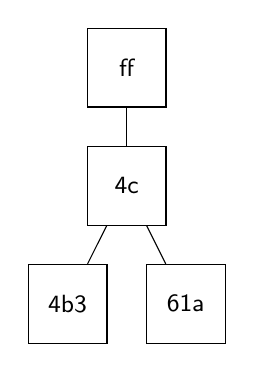
\begin{tikzpicture}[
  every node/.style={font=\sffamily\small, draw, rectangle, minimum size=10mm, align=center},
  -, >=stealth
]

\node (root1) {ff}
    child {node {4c}
      child {node {4b3}}
      child {node {61a}}
    };
\end{tikzpicture}
\caption{organization of files under the folder \texttt{ff}, represented as a tree structure.}
\label{fig:file-organization-example-in-tree}
\end{figure}

From this figure, the reader can observe that \texttt{4c} can be regarded as an internal node with two leaves. For a larger example, Figure \ref{fig:file-organization-example-in-tree-2} shows how the same organization scales when more files are stored in the folder \texttt{ff}. At this scale, the overall structure resembles a larger tree with \texttt{ff} as the root.  

It is important to clarify, however, that the diagrams so far represent \emph{directory trees}, not Merkle trees. In a Merkle tree, internal nodes are not simply folders but cryptographic hashes computed from their children (the leaves or subtrees). For this reason, the second-level folders in the figure cannot directly be considered internal nodes of a single Merkle tree. Instead, the entire filesystem should be viewed as a \emph{Merkle tree forest}: each second-level folder forms an independent Merkle tree, while each top-level folder can itself be treated as a Merkle tree whose leaves are the root hashes of its subfolders.

\begin{figure}[h]
\centering
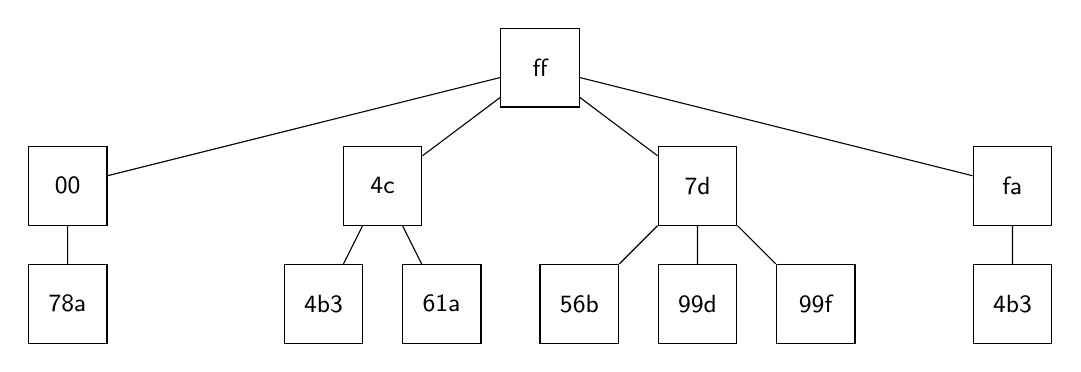
\begin{tikzpicture}[
  every node/.style={font=\sffamily\small, draw, rectangle, minimum size=10mm, align=center},
  level 1/.style={sibling distance=40mm, level distance=15mm},
  level 2/.style={sibling distance=15mm, level distance=15mm},
  -, >=stealth
]

\node (root1) {ff}
    child {node {00}
      child {node {78a}}
    }
    child {node {4c}
      child {node {4b3}}
      child {node {61a}}
    }
    child {node {7d}
      child {node {56b}}
      child {node {99d}}
      child {node {99f}}
    }
    child {node {fa}
      child {node {4b3}}
    };
\end{tikzpicture}
\caption{Extended example of file organization under \texttt{ff}, represented as a tree structure with multiple files.}
\label{fig:file-organization-example-in-tree-2}
\end{figure}

If the leaves of a Merkle tree correspond to individual file blocks or shards, then a single root hash can represent the entire \texttt{ff} folder. Alternatively, smaller Merkle trees can be built independently for each subfolder. For instance, in Figure \ref{fig:file-organization-example-in-tree-2}, one could compute four Merkle root hashes for the second-level folders and one root hash for the top-level folder \texttt{ff}.

This arrangement, referred to here as a \emph{Merkle tree forest}, allows up to 256 top-level folders. Since only lowercase hexadecimal strings are used, ensuring compatibility with both case-sensitive and case-insensitive filesystems, the range spans from \texttt{00/} to \texttt{ff/}. Each top-level folder can contain up to 256 second-level folders, as the namespace is determined by four hexadecimal characters. Dividing the data into smaller trees is crucial for scalable and efficient verification, as will be detailed in the following section.

\subsection{Storing different Merkle trees for each agent}

Because each file is split into $n+k$ shards and distributed across different nodes, each agent maintains its own local file organization. As a result, there are effectively $n+k$ distinct filesystems, one for each agent. It should be noted that the sets of files stored by different agents may not be identical, since some agents may be offline during an upload. Nevertheless, the file is still successfully stored thanks to the Reed-Solomon requirements.

To better understand this, we can consider the entire filesystem of an agent as a tree structured as follows:
\begin{itemize}
    \item \textbf{Root.} The global root, representing all files stored by the agent. In practice, this is rarely used because computing a Merkle tree for this element would require hashing the entire filesystem at once.
    \item \textbf{Second level.} The top-level folders (e.g., \texttt{ff}), each of which corresponds to the root of a Merkle tree for that folder.
    \item \textbf{Third level.} The second-level (or \emph{sub}) folders (e.g., \texttt{ff/4c}), which are smaller Merkle trees containing only a subset of files.
    \item \textbf{Leaves.} The actual file data blocks.
\end{itemize}

The global root of the entire filesystem is avoided because it is too expensive to compute, especially across multiple agents that may be offline at any given time. At the other extreme, while each file could theoretically be validated individually, storing and checking a hash for every file would reduce the system to a simple checksum-based corruption detection scheme, which lacks scalability.  

Instead, the system leverages intermediate Merkle trees at the \emph{folder levels}. These allow integrity verification to be performed at different granularities: either locally within a subfolder or globally within a top-level folder, without the overhead of recalculating the root hash for the entire agent's filesystem.

Figure \ref{fig:merkle-tree-filesystem-for-3-agents} illustrates an example of this organization for a Reed-Solomon configuration with $n=2, k=1$. In this example, the top-level and second-level folders are highlighted with lighter and darker colours, respectively.

For each top-level folder, every agent computes and stores the Merkle root hash obtained from a Merkle tree whose leaves correspond to the \emph{terminal files}. The same procedure is applied to second-level folders. For example, in Figure \ref{fig:merkle-tree-filesystem-for-3-agents}, Agent 1 computes and stores the Merkle root hashes of \texttt{fe}, \texttt{ff}, \texttt{fe/2d}, \texttt{ff/4c}, and \texttt{ff/6d}. Agents 2 and 3 follow the same procedure, maintaining the root hashes corresponding to their respective local filesystems.

A key property of these Merkle root hashes is that they can themselves be used as input for higher-level Merkle trees. The system computes aggregated Merkle trees from the folder roots and stores only the resulting root hashes in \textit{string format}. This recursive organization is illustrated in Figures \ref{fig:merkle-tree-first-level-of-saved-hashes} and \ref{fig:merkle-tree-second-level-of-saved-hashes}.

The distinction between top-level and second-level folder roots becomes largely irrelevant in storage terms: both are represented uniformly in a map, where the key is the folder identifier (two characters for a top-level folder, five for a second-level folder) and the value is the corresponding root hash. This raises a couple of questions: which component is responsible for storing and maintaining this map, and why does the system use two levels of folders instead of just one?

\begin{figure}[H]
\centering
\begin{tikzpicture}[
  every node/.style={font=\sffamily\small, draw, rectangle, minimum size=10mm, align=center},
  greenborder/.style={draw=green!90!black, thick},
  greenborder2/.style={draw=green!50!black, thick},
  blueborder/.style={draw=cyan!90!black, thick},
  blueborder2/.style={draw=cyan!50!black, thick},
  yellowborder/.style={draw=orange!90!black, thick},
  yellowborder2/.style={draw=orange!50!black, thick},
  level 1/.style={sibling distance=55mm, level distance=15mm},
  level 2/.style={sibling distance=35mm, level distance=15mm},
  level 3/.style={sibling distance=28mm, level distance=15mm},
  level 4/.style={sibling distance=28mm, level distance=15mm},
  -, >=stealth
]

\node (root1) {Agent 1}
  child {node[greenborder] {fe}
    child {node[greenborder2] {fe/2d}
      child {node {0f8.1}}
    }
  }
  child {node[greenborder] {ff}
    child {node[greenborder2] {ff/4c}
      child {node {4b3.1}}
      child {node {61a.1}}
    }
    child {node[greenborder2] {ff/6d}
      child {node {db7.1}}
    }
  };

\node[below=6cm of root1] (root2) {Agent 2}
  child {node[blueborder] {fe}
    child {node[blueborder2] {fe/2d}
      child {node {0f8.2}}
    }
  }
  child {node[blueborder] {ff}
    child {node[blueborder2] {ff/4c}
      child {node {4b3.2}}
      child {node {61a.2}}
    }
    child {node[blueborder2] {ff/6d}
      child {node {db7.2}}
    }
  };

\node[below=6cm of root2] (root3) {Agent 3}
  child {node[yellowborder] {fe}
    child {node[yellowborder2] {fe/2d}
      child {node {0f8.3}}
    }
  }
  child {node[yellowborder] {ff}
    child {node[yellowborder2] {ff/4c}
      child {node {4b3.3}}
      child {node {61a.3}}
    }
    child {node[yellowborder2] {ff/6d}
      child {node {db7.3}}
    }
  };

\end{tikzpicture}
\caption{Example of filesystems for \texttt{Agent 1}, \texttt{Agent 2}, and \texttt{Agent 3}.}
\label{fig:merkle-tree-filesystem-for-3-agents}
\end{figure}


\begin{figure}[H]
\centering
\begin{tikzpicture}[
  every node/.style={font=\sffamily\small, draw, rectangle, minimum size=10mm, align=center},
  hash1/.style={draw=green!90!black, thick},
  hash2/.style={draw=cyan!90!black, thick},
  hash3/.style={draw=orange!90!black, thick},
  level distance=15mm,
  sibling distance=50mm,
  <-, >=stealth
]

%%%% First graph: fe at top, hashes below
\node (fe) {\texttt{fe}}
  child {node[hash1] {\texttt{fe}'s root of Agent 1}}
  child {node[hash2] {\texttt{fe}'s root of Agent 2}}
  child {node[hash3] {\texttt{fe}'s root of Agent 3}};

%%%% Second graph: ff at top, hashes below
\node[below=2cm of fe] (ff) {\texttt{ff}}
  child {node[hash1] {\texttt{ff}'s root of Agent 1}}
  child {node[hash2] {\texttt{ff}'s root of Agent 2}}
  child {node[hash3] {\texttt{ff}'s root of Agent 3}};

\end{tikzpicture}
\caption{Merkle tree constructed from the root hashes of top-level folders. Each folder root acts as a leaf in this Merkle tree.}
\label{fig:merkle-tree-first-level-of-saved-hashes}
\end{figure}

\begin{figure}[H]
\centering
\begin{tikzpicture}[
  every node/.style={font=\sffamily\small, draw, rectangle, minimum size=10mm, align=center},
  hash1/.style={draw=green!50!black, thick},
  hash2/.style={draw=cyan!50!black, thick},
  hash3/.style={draw=orange!50!black, thick},
  level distance=15mm,
  sibling distance=50mm,
  <-, >=stealth
]

%%%% First graph: fe at top, hashes below
\node (fe/2d) {\texttt{fe/2d}}
  child {node[hash1] {\texttt{fe/2d}'s root of Agent 1}}
  child {node[hash2] {\texttt{fe/2d}'s root of Agent 2}}
  child {node[hash3] {\texttt{fe/2d}'s root of Agent 3}};

%%%% Second graph: ff at top, hashes below
\node[below=2cm of fe/2d] (ff/4c) {\texttt{ff/4c}}
  child {node[hash1] {\texttt{ff/4c}'s root of Agent 1}}
  child {node[hash2] {\texttt{ff/4c}'s root of Agent 2}}
  child {node[hash3] {\texttt{ff/4c}'s root of Agent 3}};
  
\node[below=2cm of ff/4c] (ff/6d) {\texttt{ff/6d}}
  child {node[hash1] {\texttt{ff/6d}'s root of Agent 1}}
  child {node[hash2] {\texttt{ff/6d}'s root of Agent 2}}
  child {node[hash3] {\texttt{ff/6d}'s root of Agent 3}};

\end{tikzpicture}
\caption{Merkle tree constructed from the root hashes of second-level folders. Each folder root acts as a leaf in this Merkle tree.}
\label{fig:merkle-tree-second-level-of-saved-hashes}
\end{figure}

\newpage
